% Тут используется класс, установленный на сервере Papeeria. На случай, если
% текст понадобится редактировать где-то в другом месте, рядом лежит файл matmex-diploma-custom.cls
% который в момент своего создания был идентичен классу, установленному на сервере.
% Для того, чтобы им воспользоваться, замените matmex-diploma на matmex-diploma-custom
% Если вы работаете исключительно в Papeeria то мы настоятельно рекомендуем пользоваться
% классом matmex-diploma, поскольку он будет автоматически обновляться по мере внесения корректив
%

% По умолчанию используется шрифт 14 размера. Если нужен 12-й шрифт, уберите опцию [14pt]
%\documentclass[14pt]{matmex-diploma}
\documentclass[14pt]{matmex-diploma-custom}
\usepackage{mwe}
\usepackage{caption}    % -> Подписи
\usepackage{subfig}     % -> Позволяет ставить фигуры рядом
\usepackage{hyperref}   % -> Удобные ссылки

\begin{document}
% Год, город, название университета и факультета предопределены,
% но можно и поменять.
% Если англоязычная титульная страница не нужна, то ее можно просто удалить.
\filltitle{ru}{
    chair               = {Математическое обеспечение и администрирование \\ информационных систем},
    title               = {Разработка сервиса для заказа еды},
    % Здесь указывается тип работы. Возможные значения:
    %   coursework      - Курсовая работа
    %   diploma         - Диплом специалиста
    %   master          - Диплом магистра
    %   bachelor        - Диплом бакалавра
    %   report          - Отчёт по учебной практике (первый/второй курс)
    type                = {report},
    position            = {студента},
    group               = 244,
    author              = {Липаев Савелий Витальевич},
    supervisorPosition  = {к.\,т.\,н.,},
    supervisor          = {Литвинов Ю.\,В.},
    % university          = {Санкт-Петербургский Государственный Университет},
    % faculty             = {Математико-механический факультет},
    % city                = {Санкт-Петербург},
    % year                = {2020}
}
\maketitle
\tableofcontents

% У введения нет номера главы
\section*{Введение}
	Обучаясь в любом вузе страны, студенты должны иметь возможность полноценно питаться.
	В большинстве учебных заведений существуют свои столовые, которые находятся в учебном корпусе или по соседству на территории учебного заведения.

	Когда студенты приходят поесть в перерыве между занятиями, возникает огромная очередь, а во время занятий в столовой почти не бывает посетителей.
	В результате многие студенты перестают посещать такие столовые из-за нежелания тратить время в очереди, а потом есть в спешке — столовая теряет прибыль,
	студент либо остаётся голодным, либо с большой вероятностью опаздывает на следующую пару.

	Создание мобильного приложения (или даже онлайн сервиса) для предварительного заказа еды в студенческих столовых, позволило бы эффективно решить вышеописанные проблемы.
	% кратко про REST нач.
	Обычно такие сервисы используют архитектуру \textit{\textbf{клиент — сервер}}, где в качестве \textit{клиента} выступает мобильное приложение, а \textit{серверная часть} представлена в виде RESTful API \footnote{RESTful — значит не нарушающих принципов архитектуры REST}.
	% кратко про REST конец.

	Как показывает статистика \cite{russian_ecommerce_market}, популярность таких сервисов растёт вместе с рынком электронной коммерции в России.
	Мобильное приложение было бы востребовано среди студентов, в силу удобства использования, а изолированный от клиента, API позволил бы использовать приложение для столовых различных учебных заведений.

	Все эти причины побудили авторов отчёта к созданию такого сервиса, под рабочим названием <<Project Stolovka>> (далее пр. Stolovka).

\section{Постановка задачи}
	Проект разрабатывался совместно с Виктром Ховановым \footnote{https://github.com/m0rphed}.
	Общая цель проекта: создание сервиса для заказа еды, с узкой специализацией – столовые вузов.
	Выбранный подход к разработке такого сервиса предполагает два основных программных модуля:
	\begin{description}
	    \item[Мобильное приложение] — предоставляет пользователю удобный единообразный интерфейс на самых популярных мобильных платформах — Android и iOS\footnote{По данным 2018 года: Android занимает ок. 86\%  от всех мобильных ОС~\cite{gartner_mobile_os_share}}.
	    \item[RESTful API] — обеспечивает доступ к данным пользователей (осуществляет CRUD операции БД) через HTTP запросы по сети, что позволяет полностью разделить клиент и сервер, а также позволяет увеличить производительность даже при относительно большом количестве запросов.
	\end{description}
	Соответственно, для достижения вышеописанных целей были поставлены следующие задачи:
	\begin{itemize}
	    \item Создание простого мобильного интерфейса, подходящего для предметной области
	    \item Разработка мобильного приложения для предварительного заказа еды: на определённое время, в конкретной столовой
	    \item Создание RESTful API на ASP.NET Core \cite{rest_xamarin}
	    \item Проектирование и реализация базы данных
	    \item Следование современным стандартам разработки ПО
	    \item Применение практик DevOps и Continuous Integration для поддержания проекта в рабочем состоянии на протяжении всего цикла разработки
	    \item Написание веб-клиента для кассиров, работников столовой.
	\end{itemize}
	За разработку мобильного приложения, а также части API, был ответственен Савелий Липаев. Его задачами были:
	\begin{itemize}
	    \item проектирование архитектуры моб. приложения
	    \item реализация пользовательского интерфеса Material Design
	    \item разработка бизнес-логики моб. приложения
	    \item реализация аутентификации пользователей, используя протокол OAuth 2.0
	    \item обеспечение связи между приложением и API
	    \item написание контроллеров ASP.NET Core API для обработки HTTP-запросов, поступающих от приложения
	\end{itemize}
	Хованову Виктору были поручены следующие задачи:
	\begin{itemize}
	    \item разработка макета UI для моб. приложения
	    \item проектирование архитектуры серверной части
	    \item проектирование схемы базы данных
	    \item администрирование сервера, отладка API
	    \item интеграция c Docker
	\end{itemize}

\section{Обзор существующих решений}
	Самыми близкими аналогами являются приложения кафе и ресторанов,
	предоставляющие пользователю возможность заказывать еду удалённо.

	Рассмотрим подробнее {\bf мобильные интерфесы} близких аналогов пр. Stolovka, выделим некоторые удачные и неудачные идеи:
	\paragraph{Столовая Поварёшка}
	    \begin{itemize}
	        \item[+] Интуитивный, не перегруженный пользовательский интерфейс
	        \item[-] Узко специализированный, только для одной сети столовых
	        \item[-] Нет приложений для всех мобильных платформ, только Android
	    \end{itemize}
	    Большим достоинством этого приложения является простой интерфейс.
	    Поскольку изначально задумка пр. Stolovka ориентирована на студентов, удобство и простота использования приложения является важным фактором.
	\paragraph{Сытый офис}
	    \begin{itemize}
	        \item[+] Есть приложение для всех мобильных устройств
	        \item[-] Неадаптированно для студентов и столовых
	    \end{itemize}
	    В этом приложении очень удачно реализована возможность выбора меню в зависимости от дня недели (см. ~\ref{fig:other_ui}).
	    Это было бы особенно удобно именно для столовых, поскольку во многих из них меню зависит от дня недели.
	    \newpage
	\paragraph{Мобильное приложение ДоДо Пицца}
	    \begin{itemize}
	        \item[+] Удобное управление корзиной с мобильного устройства
	        \item[+] Мобильное для iOS, Android
	        \item[-] Сервис ориентирован только на сеть DoDo, нет возможности интеграции
	    \end{itemize}
	    \begin{figure}[ht!]
	        \subfloat[Столовая Поварёшка]{
	            \begin{minipage}[t]{0.3\textwidth}
	                \centering
	                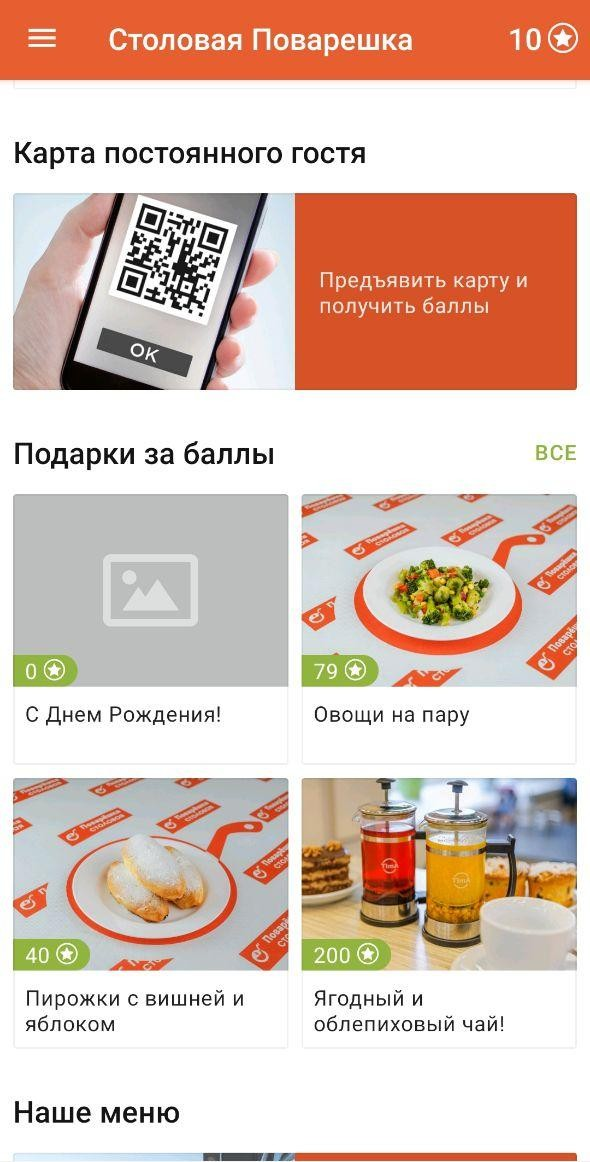
\includegraphics[width=\textwidth]{images/ui_screen_01.jpg}
	            \end{minipage}}
	        \hfill
	        \subfloat[Cытый Офис]{
	            \begin{minipage}[t]{0.3\textwidth}
	                \centering
	                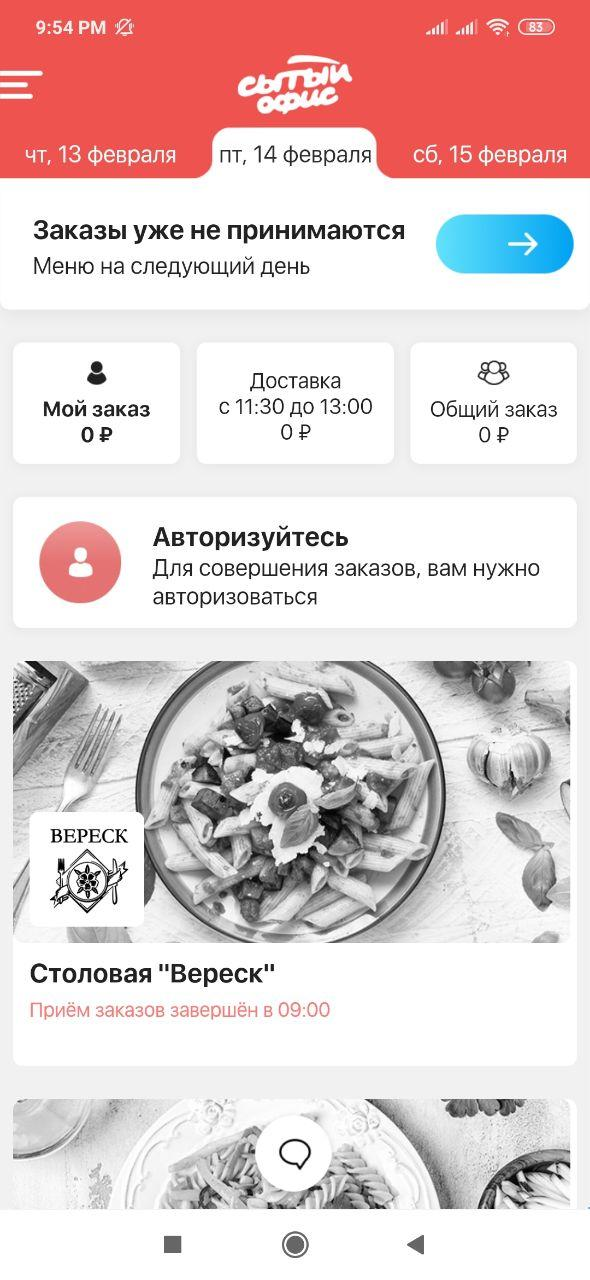
\includegraphics[width=\textwidth]{images/ui_screen_02.jpg}
	            \end{minipage}}
	        \hfill
	        \subfloat[ДоДо Пицца]{
	            \begin{minipage}[t]{0.3\textwidth}
	                \centering
	                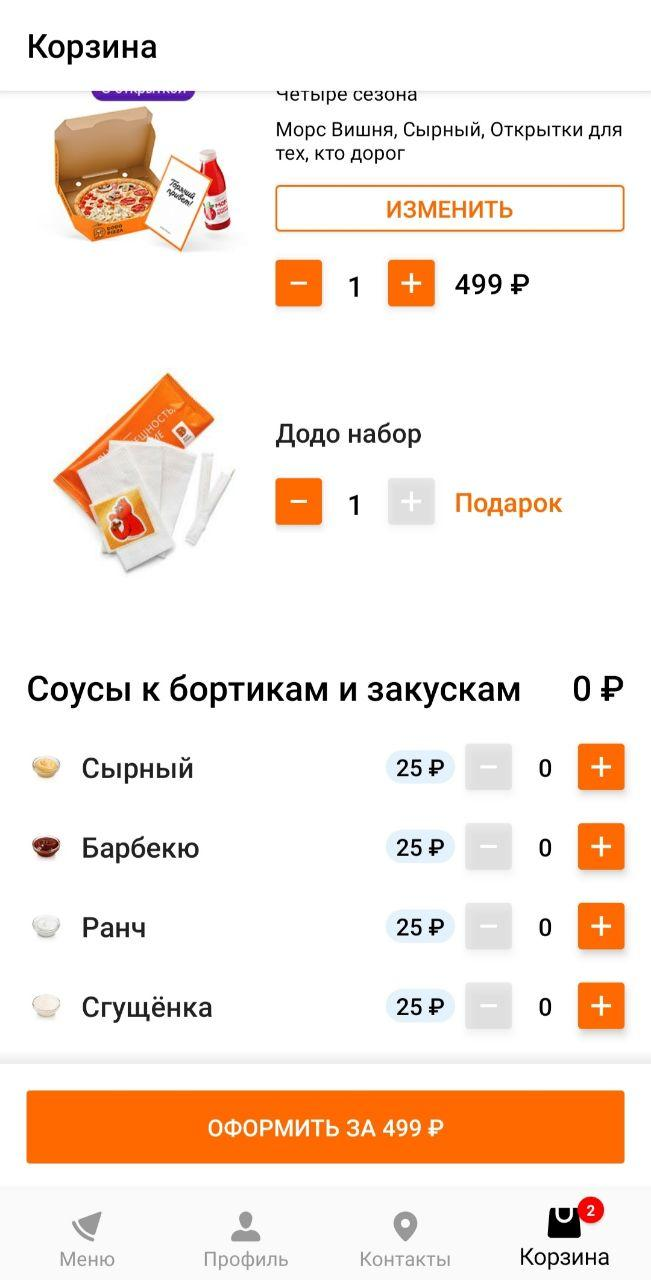
\includegraphics[width=\textwidth]{images/ui_screen_03.jpg}
	            \end{minipage}}
	        \caption{Приложения-аналоги}
	        \label{fig:other_ui}
	    \end{figure}
	    Каждое из рассмотренных приложений имеет свои интересные решения, однако, в отличии от пр. Stolovka эти приложения обычно не предоставляют API, чаще всего они привязаны к конкретному бренду, не адаптированы для студентов.
	    Проанализировав распространенные приложения, стало понятно, что следует сосредоточиться на разработке {\it открытого API}, а мобильное приложение должно иметь более простой, но вместе с тем знакомый пользователю, интерфейс.
	    Опираясь на анализ пользовательских интерфейсов был составлен макет в программе Figma\footnote{Макет UI доступен по ссылке: https://bit.ly/3cp66U}.

\section{Реализация}
	\subsection{Архитектура}
	    Проект {\it Stolovka} включает в себя мобильное приложение (далее {\bf \it клиент}) работающее в связке с RESTfull API, которое осуществляет обработку запросов, и посредством взаимодействия с базой данных обеспечивает отслеживание текущих заказов в реальном времени для каждого пользователя.

	    REST определяет ряд архитектурных принципов проектирования Web-сервисов, ориентированных на системные ресурсы, включая способы обработки и передачи состояний ресурсов по HTTP разнообразными клиентскими приложениями, написанными на различных языках программирования.

	\subsection{Мобильное приложение Xamarin.Forms}
	    В качестве основного фреймворка для написания мобильного приложения использовался Xamarin.Forms (далее XF).
	    Упор был сделан на разработку под Android, т.к. протестировать iOS приложение, не обладая устройством Apple затруднительно.

	    Приложение, написанное на XF, имеет единую логику для всех мобильных платформ, написанную на языке C\#,
	    также он позволяет писать единый пользовательский интерфейс (далее UI) для всех платформ с помощью языка разметки XAML.

	    \begin{figure}[h!]
	        \centering
	        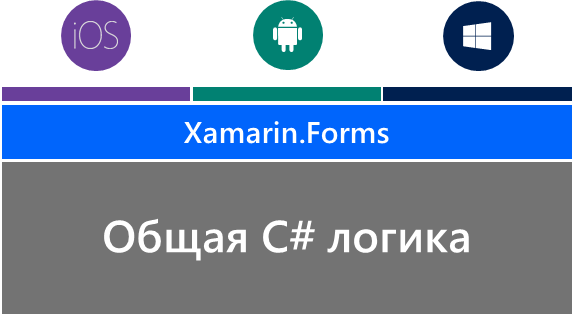
\includegraphics[scale=0.7]{images/xamarin_forms_framework}
	        \caption{Xamarin.Forms App Architecture}
	        \label{fig:xf_app_arch}
	    \end{figure}

	    Однако, разработчик также может реализовать UI нативно (частично или полностью).
	    Поскольку всё компилируется в нативный код мобильных платформ, приложения, написанные на XF
	    имеют высокую производительность очень близкую к нативной, а иногда и выше\footnote{Performance Comparison: Xamarin.Forms, Xamarin.iOS, Xamarin.Android vs Android and iOS \cite{xamarin_perf_vs_native}}.

	    В качестве архитектурного паттерна использовался \\ Model-View-ViewModel(MVVM)\cite{MVVM_wiki},
	    позволяющий удобно разделить бизнес-логику и UI.

	    MVVM является самым распространенным архитектурным паттерном для XF.

	    Для авторизации в приложение использовался открытый протокол авторизации OAuth 2.0, позволяющий мобильному приложению получать ограниченный доступ к аккаунту пользователя на различных сервисах.

	    Т.к. приложение поддерживает протокол OAuth 2.0, пользователь может не тратить время на регистрацию и подтверждение аккаунта, вместо этого он может использовать для входа аккаунты Google или ВКонтакте (см. рис. ~\ref{fig:stolovka_ui}).

	    Работает это следующим образом:
	    \begin{enumerate}
	        \item Приложение переадресовывает на страницу авторизации сервиса;
	        \item Пользователь авторизуется и подтверждает выдачу прав;
	        \item Сервис переадресовывает обратно в приложение, передавая приложению authorization code;
	        \item Приложение отправляет POST запрос, содержащий authorization code, в результате которого получает access token;
	        \item С помощью токена приложение получает данные о пользователе, доступ к которым пользователь разрешил ранее;
	    \end{enumerate}

	    \begin{figure}[h!]
	        \subfloat[Экран входа]{
	            \begin{minipage}[t]{0.3\textwidth}
	                \centering
	                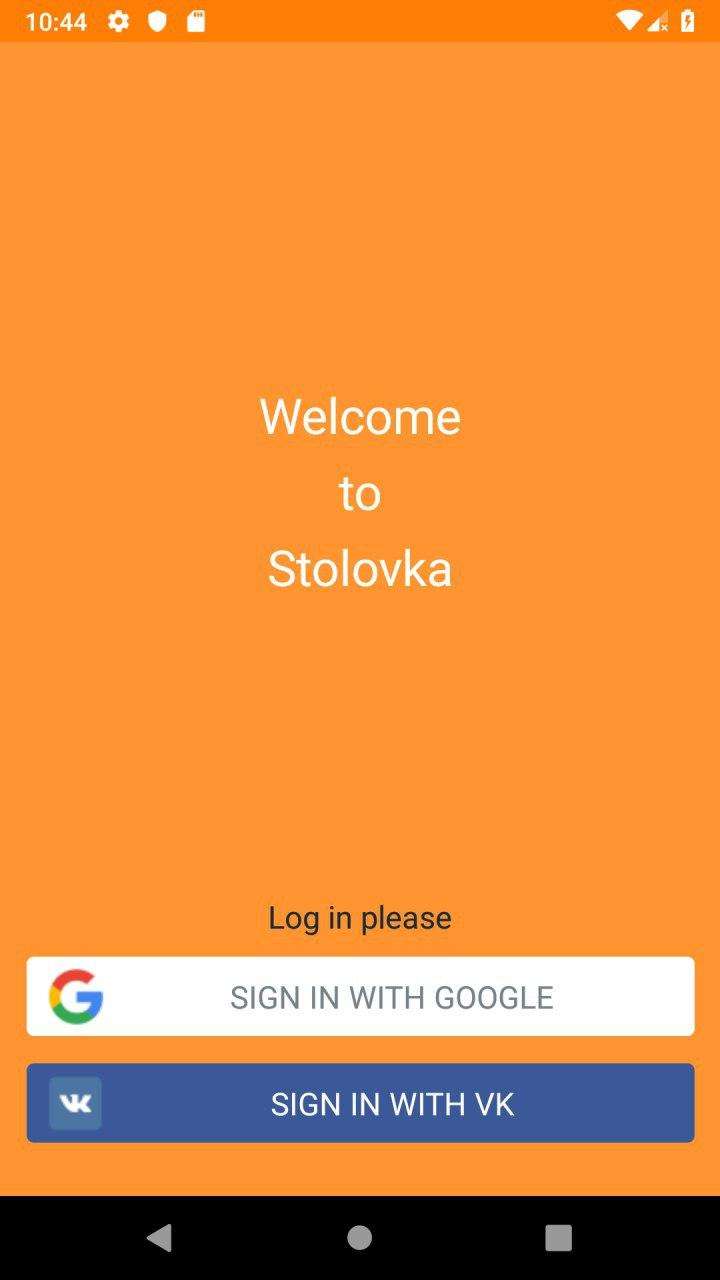
\includegraphics[width=\textwidth]{images/stolovka_login}
	            \end{minipage}}
	        \hfill
	        \subfloat[Экран меню]{
	            \begin{minipage}[t]{0.3\textwidth}
	                \centering
	                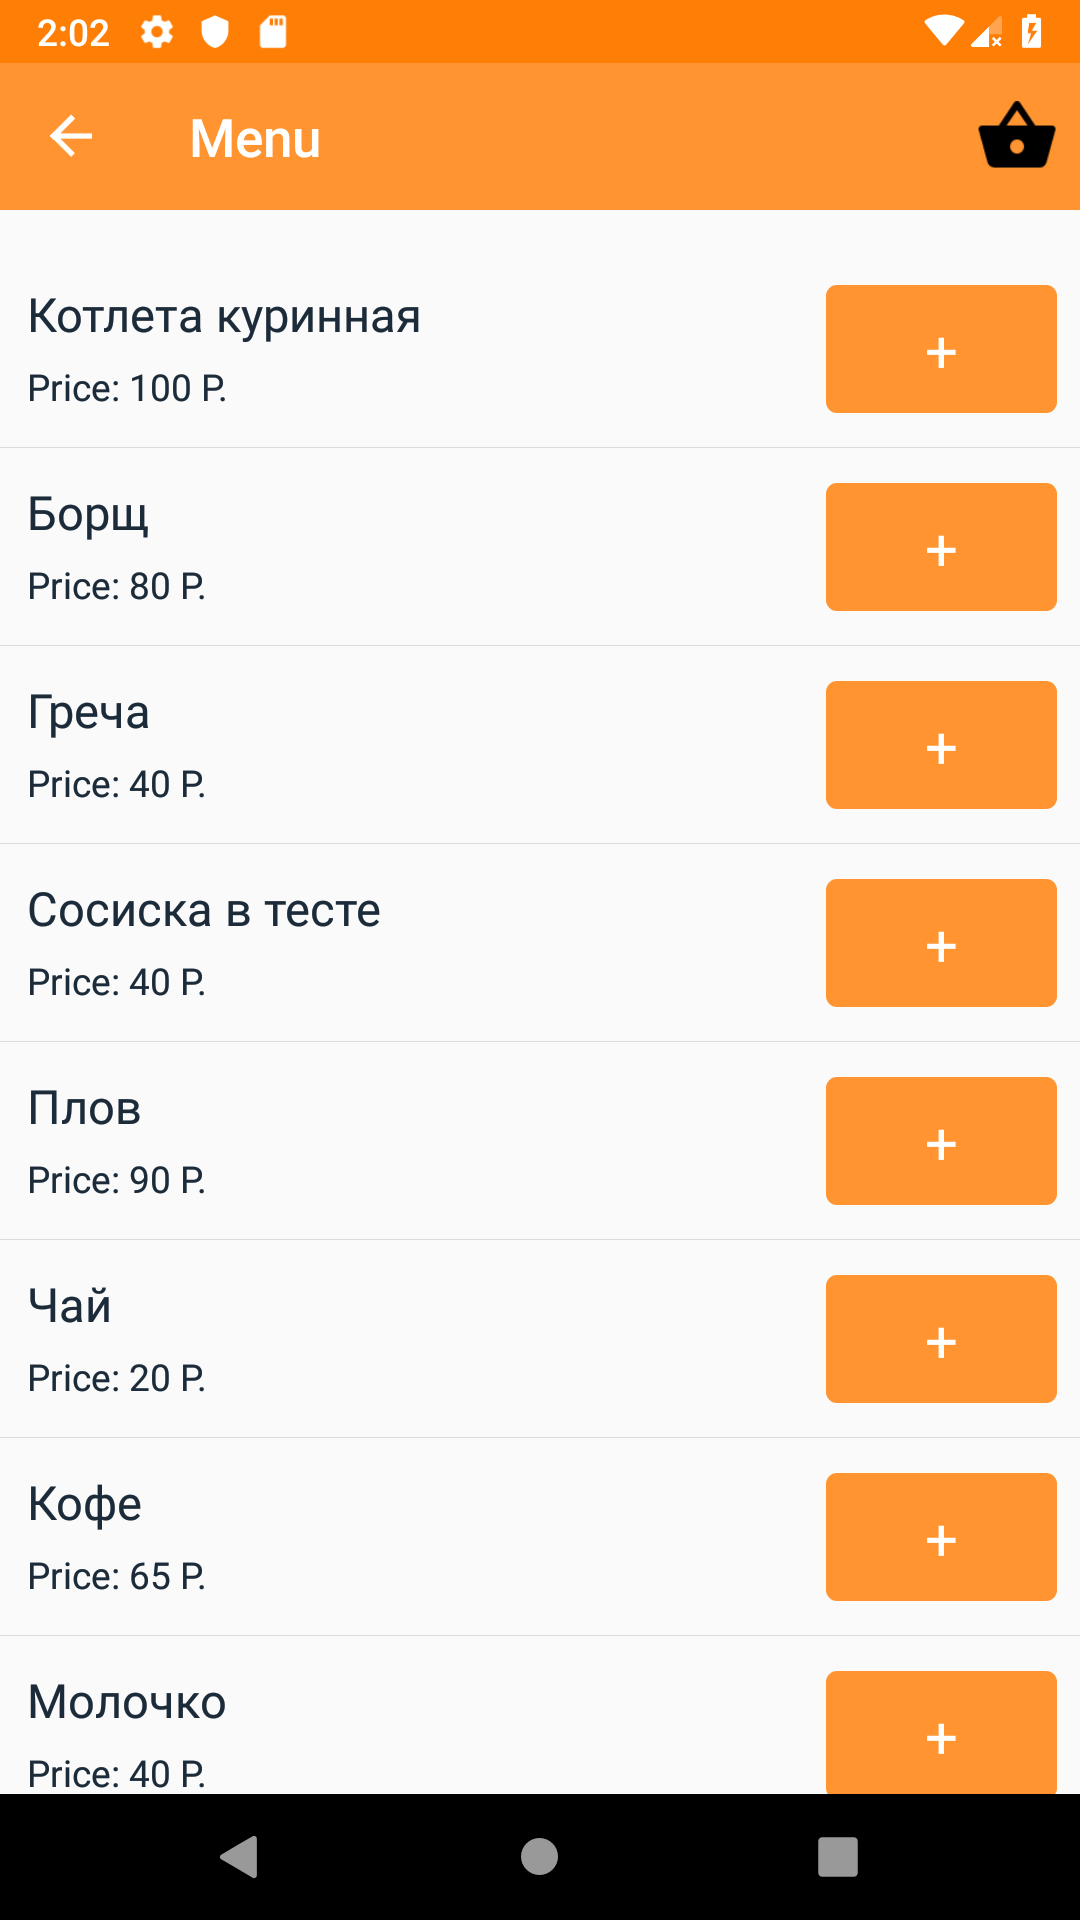
\includegraphics[width=\textwidth]{images/stolovka_screen_02}
	            \end{minipage}}
	        \hfill
	        \subfloat[Интерфейс корзины]{
	            \begin{minipage}[t]{0.3\textwidth}
	                \centering
	                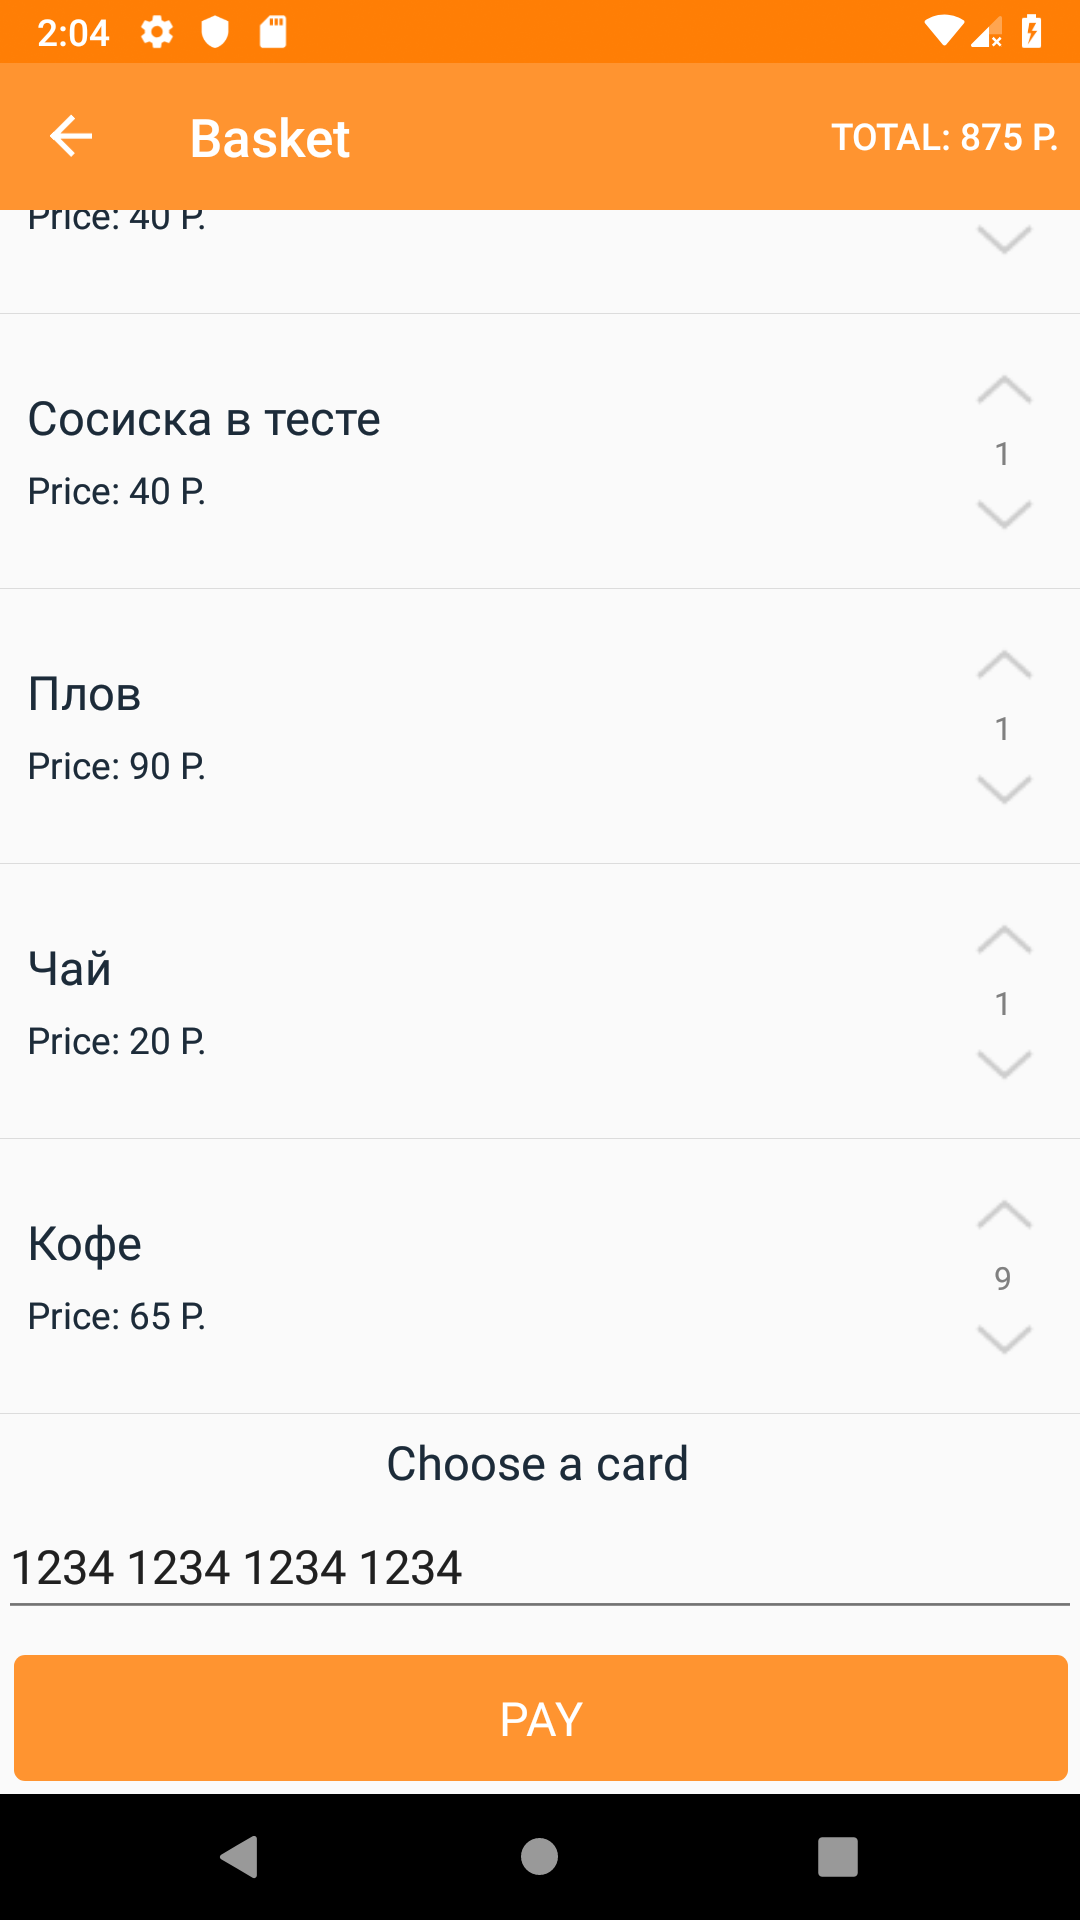
\includegraphics[width=\textwidth]{images/stolovka_screen_03}
	            \end{minipage}}
	        \caption{Приложение Stolovka v 1.0}
	        \label{fig:stolovka_ui}
	    \end{figure}

	    Для взаимодействия с RESTful API использовалась библиотека Refit, позволяющая легко описывать спецификацию в виде интерфейса с понятными входными и выходными параметрами, а также предоставляющая возможность манипулировать HTTP-заголовками для отдельных запросов.

	    При разработке мобильных приложений работающих необходимо также учитывать нестабильное соединение с сетью.
	    Соответственно, возникает необходимость повторного выполнения запросов, не перегружая пользователя дополнительными просьбами повторить действие.
	    Поэтому, для обработки неудачных сетевых запросов используется библиотека \textbf{Polly}\cite{polly_github}.

	    Для кэширования информации о пользователе использовалось хранилище Akavache\cite{akavache_github}, работающее как {\it обёртка} над БД SQLite.
	    Стоит отметить, что для кэширования можно было использовать другие мобильные СУБД (например Realm).
	    Однако, другие библиотеки были не настолько просты в использовании по сравнению с Akavache и обладали избыточной функциональностью.

	\subsection{ASP.NET Backend}
	    Каждого пользователю необходимо авторизовать в приложении, чтобы иметь возможность оплачивать заказ, а также подтвердить оплату.
	    Для этого существуют различные способы аутентификации, самым распространённый, а также наиболее безопасным решением является использование JSON Web Tokens.

	    \subsubsection{Аутентификаци и авторизация: JWT и ASP.NET Identity}
	        JSON web tokens — это стандарт кодирования данных, включающий в себя информацию о роли (т.е. правах доступа) пользователя и другие данные, относящиеся к вашему сайту.

	        JWT предлагает безопасный метод отправки этой информации с использованием общего секретного ключа.
	        Разные эндпойнты могут требовать разных ролей, с перенаправленнием на другие страницы при неудачной аутентификации.

	        Роль пользователя для управления содержимым и контроля пользовательских возможностей.

	    \subsubsection{База данных}
	        \begin{figure}
	            \centering
	            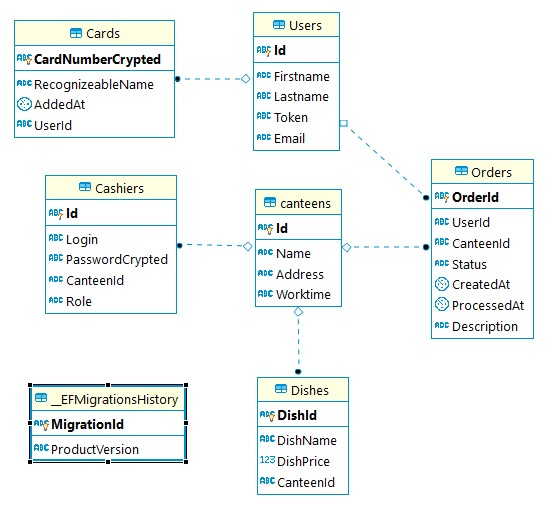
\includegraphics[scale=0.8]{images/database_arch_01.jpg}
	            \caption{Схема базы данных}
	            \label{db_arch}
	        \end{figure}
	        Для работы с СУБД PostgreSQL на бэкенде используется Entity Framework Core ~\cite{npgsql_efcore_doc},
	        схема базы данных представлена на рисунке ~\ref{db_arch}.

	        Для оптимизации запросов к RESTful API используется кэширование с помощью mem-cache базы данных Redis\cite{redis_doc}.

	    \subsubsection{CI и DevOps проекта}
	        Для того, чтобы легко обновлять сервисы и разворачивать их на серверах, в больших командах принято следовать методологии Continuous Integration(далее CI).

	        С практической точки зрения это значит, что в любой момент времени должна быть полностью работающая актуальная версия продукта, которую можно протестировать или продемонстрировать.
	        \begin{enumerate}
	            \item Автоматические ежедневные сборки
	            \item Уведомления о проблемах
	            \item Интеграцию с баг-трекером и системой контроля версий
	            \item Версионирование продукта — каждый продукт
	            \item Версионирование базы данных
	            \item Автоматизированные выкладки и резервные копии
	        \end{enumerate}

	        Для автоматизации тестирования использовался AppVeyor и TravisCI что позволяло сразу же во время разработки получить готовую сборку проекта.

	    \subsubsection{Документирование API c помощью Swagger}
	        Стоит уточнить, что REST архитектура не задаёт в явном виде как должен выглядет конкретный запрос к API.
	        Однако, существуют способы единообразного описания путей к сущностям из базы данных — можно представлять это как некоторую грамматику запросов — всё это называется \textit{REST endpoints}. В API это реализовано следующим образом:
	        Для указания пути к коллекции просто используется название соответствующей сущности, если это список пользователей, то путь будет таким: \textbf{/users}.
	        В запросах на получение списков мы можем использовать множество дополнительных параметров, но они должны быть опциональными, т.е. параметры не передаются как часть пути.

	        Пример: \textrm{GET /api/v1/users/25/name}

	        У открытого API должна быть документация, в противном случае поддерживать его будет затруднительно для большой команды, \\ а использование API разработчиками сторонних сервисов будет невозможно.

	        Для генерации документации хорошо подходит фреймворк Swagger, который так же предоставляет удобный WEB интерфейс для тестирования API.

	        В нашем проекте Swagger используется как изолированный сервис (nuget-пакет внутри ASP.NET API), Swagger генерирует документацию в формате HTML для всех \textit{REST endpoints}.
	        Таким образом, при добавлении нового контроллера документация будет сгенерирована автоматически.
	        \begin{figure}
	            \flushleft
	            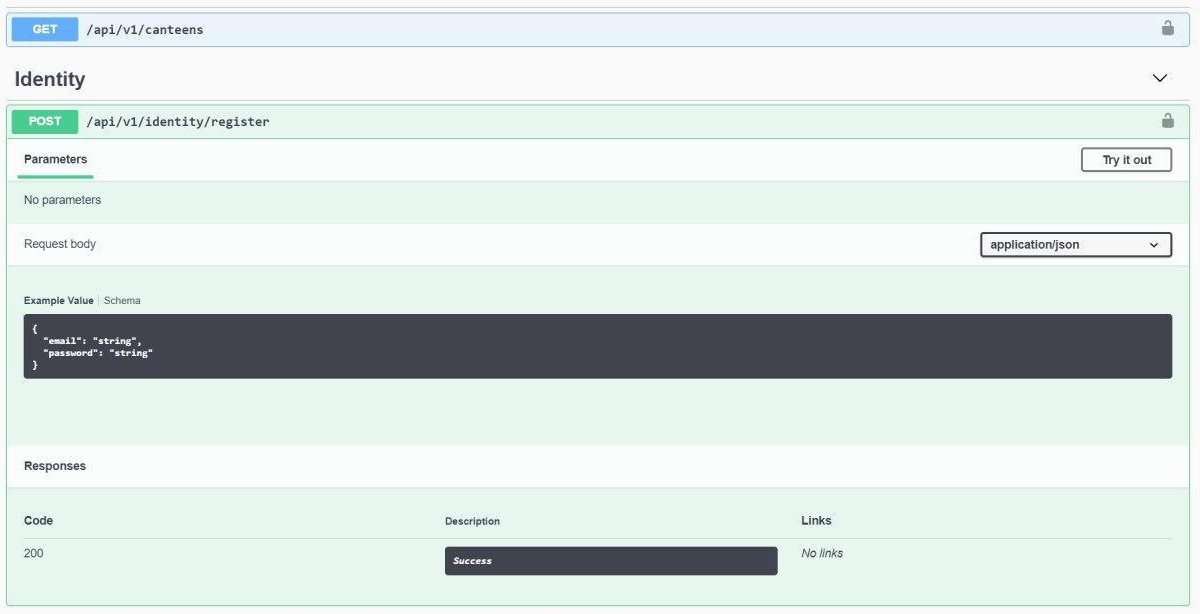
\includegraphics[scale=0.35]{images/swagger_01.jpg}
	            \caption{Swagger UI}
	            \label{swagger_01}
	        \end{figure}

\section{Результаты}
	В процессе работы над проектом удалось достигнуть следующих результатов:
	\begin{enumerate}
	    \item Получен опыт работы с фреймворком для создания мобильных приложений Xamarin.Forms
	    \item Разработано Мобильное приложение для заказа еды
	    \item Написан MVP RESTful API для получения данных
	    \item Реализован механизм аутентификации пользователей с помощью протокола OAuth 2.0
	    \item Получен опыт создания макета интерфейса мобильного приложения
	    \item Получен опыт использования СУБД PostgreSQL, а также Redis и ORM Entity Framework
	    \item Опыт настройки веб сервера + devops (docker, ci, deploy)
	\end{enumerate}

	Код-база проекта доступна на GitHub\cite{result_github}.

	\subparagraph{Дальнейшее развитие}
	    Стоит отметить, что проект находится в стадии MVP — т.е. минимального жизнеспособного продукта, и основные функции реализованы успешно.
	    Однако, за время выделенное на проект удалось реализован не все {\it желаемые} функции, поэтому планируется и дальше проект, с внесением последующих изменений.
	    Возможные пути улучшения:
	    \begin{itemize}
	        \item разработка WEB интерфейса для работников столовых и доставщиков с возможностью отслеживания заказа
	        \item оптимизация API
	        \item более подробная документация API
	        \item улучшенный пользовательский интерфейс
	        \item повышение производительности приложения под iOS
	    \end{itemize}

	    \setmonofont[Mapping=tex-text]{CMU Typewriter Text}
	    \bibliographystyle{ugost2008ls}
	    \bibliography{matmex_mywork.bib}
\end{document}
